% File: main.tex
% Author: Auto-Intern GmbH
% Manuals template

\newcommand{\fach}{Digitaltechnikpraktikum }
\newcommand{\titelname}{Versuchsprotokoll }
\newcommand{\matrikel}{2016507006 }
\newcommand{\name}{Olbrich, Marie }

\newcommand{\matrikelpartner}{2016506999 }
\newcommand{\namepartner}{Hoffmann, Manuel }

\newcommand{\versuchsbezeichnung}{DT5 }
\newcommand{\versuchsname}{Entwurf eines 3-Bit Komparators }
\newcommand{\semester}{SS17 }
\newcommand{\datum}{23.05.2017 }
\newcommand{\betreuer}{M.Sc. Kruse }
\newcommand{\dozent}{M.Sc. Richthofer }

\documentclass[a4paper, 11pt, fleqn, DIV=10, twoside, BCOR=10mm]{scrreprt}
\usepackage{diagbox}


%%%% Eingebundene Pakete %%%% 
\usepackage{xltxtra}

\usepackage{scrhack} 
\usepackage{xcolor}
\usepackage{color}
\usepackage{xfrac} % \sfrac{}{} für Brueche
\usepackage{graphicx}
\usepackage{float}
\usepackage{subcaption}
\usepackage{setspace}
\usepackage{wrapfig}
\usepackage{longtable}
\usepackage{geometry}
\usepackage{scrlayer-scrpage}
\usepackage{wallpaper}
\usepackage{ulem}
\usepackage{siunitx}
\usepackage{amsmath}
\usepackage{chngcntr}

%% Sorgt dafür, dass Kapitel neue Kapitel nicht auf einer neuen rechten Seite anfangen
\RedeclareSectionCommand[style=section,indent=0pt]{chapter}

%% Definition der Auto Intern Farben (Das AIschwarz wir im Fließtext nicht benutzt, stattdessen ist normales schwarz gesetzt (schwarze Tinte beim Druck günstiger)
\definecolor{THrot}{RGB}{228,0,30}
\definecolor{THblau}{RGB}{0,61,125}



%% Auto-Intern vereinfachte Befehle für Schriftarten
\newcommand{\mainfont}{\setmainfont{Lato-Regular.ttf}}
\newcommand{\LatoReg}{\setmainfont{Lato-Regular.ttf}}
\newcommand{\DaysOne}{\setmainfont{DaysOne-Regular.ttf}}
\newcommand{\LatoBold}{\setmainfont{Lato-Bold.ttf}}
\newcommand{\Avenir}{\setmainfont{AvenirLTStd-Book.otf}}
\newcommand{\LatoBlack}{\setmainfont{Lato-Black.ttf}}

%% Auto-Intern vereinfachte Befhele für Sprachwechsel eng - de
\newcommand{\Deutsch}{\usepackage[ngerman]{babel}
\renewcaptionname{ngerman}{\contentsname}{Inhaltsverzeichnis} % Standard: Inhaltsverzeichnis
\renewcaptionname{ngerman}{\listfigurename}{Abbildungsverzeichnis} % Standard: Abbildungsverzeichnis
\renewcaptionname{ngerman}{\listtablename}{Tabellenverzeichnis} % Standard: Tabellenverzeichnis
\renewcaptionname{ngerman}{\figurename}{Abbildung} % Standard: Abbildung
\renewcaptionname{ngerman}{\tablename}{Tabelle} % Standard: Tabelle
}


%% Auto-Intern vereinfachte Befehle für Textsatz
\newcommand{\Kursiv}[1]{\setmainfont{Lato-Italic.ttf}#1 \mainfont}
\newcommand{\Fett}[1]{\setmainfont{Lato-Bold.ttf}#1 \mainfont}
\newcommand{\FettKursiv}[1]{\setmainfont{Lato-BoldItalic.ttf}#1 \mainfont}
\newcommand{\Hoch}[1]{$^{\text{#1}}$}
\newcommand{\Tief}[1]{$_{\text{#1}}$}

%% Auto-Intern vereinfacht Befehle für Kapitel usw, um differenzierung zwischen Inhaltsverzeichnis und Text zu haben
\newcommand{\AItitlefont}{\LatoBold}
\newcommand{\Chapter}[1]{\chapter[#1]{\AItitlefont #1}}
\newcommand{\Section}[1]{\section[#1]{\AItitlefont #1}}
\newcommand{\Subsection}[1]{\subsection[#1]{\AItitlefont #1}}
\newcommand{\Subsubsection}[1]{\subsubsection[#1]{\AItitlefont #1}}
\newcommand{\Paragraph}[1]{\paragraph[#1]{\AItitlefont #1}}
\newcommand{\Subparagraph}[1]{\subparagraph[#1]{\AItitlefont #1}}

%% Einstellungen für Kopf- und Fußzeilen
\newcommand{\HeadAVier}{
\setlength{\footheight}{-1cm}
\setlength{\skip\footins}{5mm}
\setkomafont{pageheadfoot}{\setmainfont{Lato-Regular.ttf}} %Schriftart für Kopfzeile
\setkomafont{pagehead}{\setmainfont{Lato-Regular.ttf}} % Schriftart für Fußzeile
\pagestyle{scrheadings} % Seitenstil
\ihead{
\includegraphics[height=2cm]{../TemplateGraphics/Logo300.jpg}} % Innere Kopfzeile 7cm
\ohead{}
\chead{}
}


\newcommand{\ImpFootAVier}{
\ofoot{\LatoBlack \fach} % Äußere Fußzeile
\cfoot{}
\ifoot{
}}


\newcommand{\NormFoot}{
	\ifoot{\scriptsize% Innere Fußzeile
	\begin{tabular}{ll}
	\matrikel - \name\\%
	\matrikelpartner - \namepartner\\%
	Betreut durch: \betreuer
	\end{tabular}
	}
	\ofoot{\LatoBlack \fach\\ \versuchsbezeichnung \semester}
	\cfoot{\pagemark}
}

\newcommand{\EmptyFoot}{
\ifoot{}
\ofoot{}
\cfoot{}
}
%% Anderung der Schriftarten für Titelbeschriftungen
\usepackage{tocloft}
\setkomafont{disposition}{\AItitlefont\color{THblau}}  % farbe: ueberschrift
\renewcommand{\cfttoctitlefont}{\LatoBold \Large \color{THblau}}
\renewcommand{\cftpartfont}{\LatoReg}
\renewcommand{\cftchapfont}{\LatoReg}
\renewcommand{\cftsecfont}{\LatoReg}
\renewcommand{\cftsubsecfont}{\LatoReg}
\renewcommand{\cftsubsubsecfont}{\LatoReg}
\renewcommand{\cftparafont}{\LatoReg}
\renewcommand{\cftsubparafont}{\LatoReg}
\renewcommand{\cftfigfont}{\LatoReg}
%\renewcommand{\cftsubfigfont}{\LatoReg}
\renewcommand{\cfttabfont}{\LatoReg}
%\renewcommand{\cftsubtabfont}{\LatoReg}



\addtocontents{toc}{\protect\thispagestyle{scrheadings}}
\newcommand{\AVier}{
\HeadAVier
\ImpFootAVier
\AItitlefont
\addtolength{\wpYoffset}{-3cm}
\ThisCenterWallPaper{0.7}{../TemplateGraphics/Kopf.pdf}%
{\color{white}.}\\
\vspace{3.5cm}
\begin{center}
{{\huge \titelname  zu \versuchsbezeichnung} \\ \LatoReg \versuchsname\\ \vspace{40mm} durchgeführt von \\ \Fett \matrikel \LatoReg \name \\ \Fett \matrikelpartner \LatoReg \namepartner \\ im \semester am \datum \\ \vspace{10mm} Betreut durch: \betreuer \\ Dozent: \dozent}
\end{center}
\newpage
\mainfont
\NormFoot
\tableofcontents
\newpage
\setcounter{page}{1}
\ohead{\thepage}
}

\Deutsch
\begin{document} 
\AVier
\begin{center}
\chapter{Vorbereitende Aufgaben}
\section{1-Bit-Komparator}
\begin{tabular}{c||c|c||c|c|c}
Fall:&A&B&X&Y&Z\\
 & & &A>B&A=B&A<B\\
\hline
1&0&0&0&1&0\\
2&0&1&0&0&1\\
3&1&0&1&0&0\\
4&1&1&0&1&0\\
\end{tabular}
\captionof{table}{Wahrheitstabelle zum 1-Bit-Komparator}
\begin{equation}
	X:= A \wedge \overline{B}
\end{equation}
\begin{equation}
	Y:= (\overline{A} \wedge \overline{B}) \vee (A \wedge B)
\end{equation}
\begin{equation}
	Z:= \overline{A} \wedge B
\end{equation}
\vspace{10mm}

%
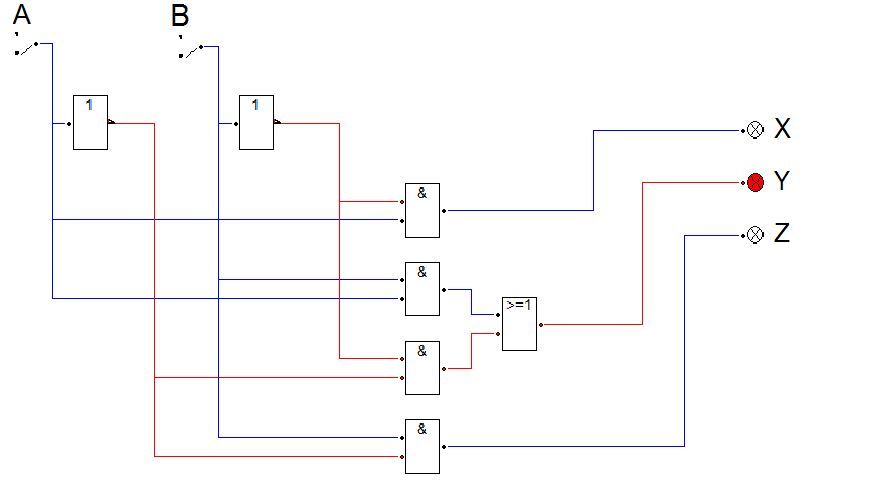
\includegraphics[width=0.9\columnwidth]{DT5Graphics/1_Bit_Komperator.jpg}
\captionof{figure}{1-Bit-Komparator}
%
\section{1-Bit-Komparator mit zusätzlichem Eingang E}
\begin{tabular}{c||c|c|c||c|c|c}
Fall:&E&A&B&X&Y&Z\\
 & & & &A>B&A=B&A<B\\
\hline
1&0&0&0&0&0&0\\
2&0&0&1&0&0&0\\
3&0&1&0&0&0&0\\
4&0&1&1&0&0&0\\
5&1&0&0&0&1&0\\
6&1&0&1&0&0&1\\
7&1&1&0&1&0&0\\
8&1&1&1&0&1&0\\
\end{tabular}
\captionof{table}{Wahrheitstabelle zum 1-Bit-Komparator mit zusätzl. Eingang E}
\begin{equation}
	X:= E \wedge A \wedge \overline{B}
\end{equation}
\begin{equation}
	Y:= (E \wedge \overline{A} \wedge \overline{B}) \vee (E \wedge A \wedge B)
\end{equation}
\begin{equation}
	Z:= E \wedge \overline{A} \wedge B
\end{equation}
\vspace{10mm}

%
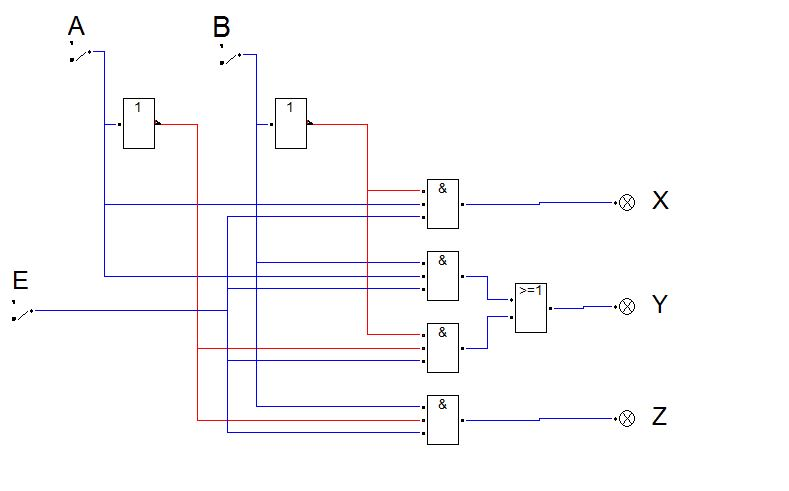
\includegraphics[width=0.9\columnwidth]{DT5Graphics/1_Bit_Komperator_mit_E.jpg}
\captionof{figure}{1-Bit-Komparator mit zusätzlichem Eingang E}
%
\section{3-Bit-Komparator}
\vspace{10mm}
\begin{tabular}{c|c|c|c|c|c|c}
Fall:&2\textsuperscript{2}&2\textsuperscript{1}&2\textsuperscript{0}&X&Y&Z\\
 &A\textsubscript{2}, B\textsubscript{2}&A\textsubscript{1}, B\textsubscript{1}&A\textsubscript{0}, B\textsubscript{0}&A>B&A=B&A<B\\
\hline
1&A\textsubscript{2}>B\textsubscript{2}&*&*&1&0&0\\
2&A\textsubscript{2}<B\textsubscript{2}&*&*&0&0&1\\
\hline
3&A\textsubscript{2}=B\textsubscript{2}&A\textsubscript{1}>B\textsubscript{1}&*&1&0&0\\
4&A\textsubscript{2}=B\textsubscript{2}&A\textsubscript{1}<B\textsubscript{1}&*&0&0&1\\
\hline
5&A\textsubscript{2}=B\textsubscript{2}&A\textsubscript{1}=B\textsubscript{1}&A\textsubscript{0}>B\textsubscript{0}&1&0&0\\
6&A\textsubscript{2}=B\textsubscript{2}&A\textsubscript{1}=B\textsubscript{1}&A\textsubscript{0}<B\textsubscript{0}&0&0&1\\
5&A\textsubscript{2}=B\textsubscript{2}&A\textsubscript{1}=B\textsubscript{1}&A\textsubscript{0}=B\textsubscript{0}&0&1&0\\
\end{tabular}
\captionof{table}{Verkürzte Wahrheitstabelle zum 3-Bit-Komparator}
\vspace{20mm}

%
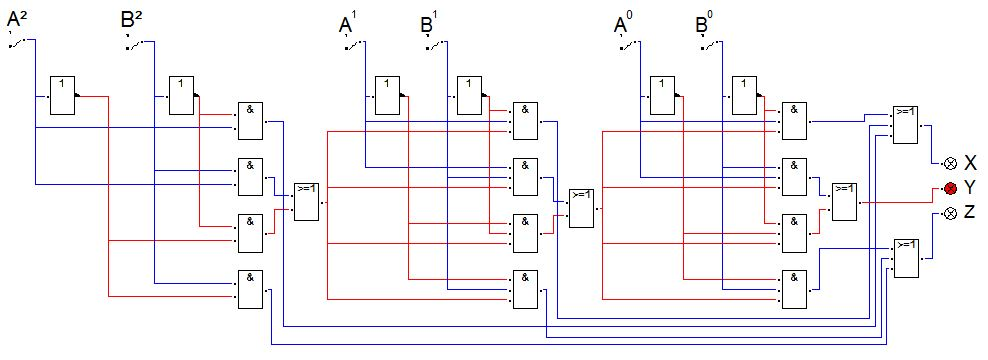
\includegraphics[width=1.25\columnwidth]{DT5Graphics/3_Bit_Komperator.jpg}
\captionof{figure}{3-Bit-Komparator}
%
\end{center}
\newpage
\chapter{Kritische Schlussbetrachtung}
\section{Olbrich, Marie}
 In Versuch DT5 sollte ein 3-Bit Komparator entworfen werden, der am Versuchstag aufzubauen und in seiner Funkton vorzuführen war. \par
Dazu sollten in den vorbereitenden Aufgaben Wahrheitstabellen zum 1-Bit-Komparator ohne und mit zusätzlichem Eingang E entwickelt werden. Anschließend war die verkürzte Wahrheitstabelle zum 3-Bit-Komparator zu entwickeln. Es ist nur die verkürzte Wahrheitstabelle verlangt, da die Tabelle ansonsten unübersichtlich lang wäre und die anderen Fälle nicht relevant sind. An Hand der Wahrheitstabellen war schließlich eine Schaltung für einen 3-Bit-Komparator zu entwerfen. \par
Die Komparatoren haben zwei oder drei Eingänge und drei Ausgänge. Zwei Eingänge dienen der Eingabe der beiden Zahlen und der optionale dritte Eingang E ist ein Sperreingang. Nur wenn eine 1 an dem Eingang anliegt, schaltet er den Komparator frei. Der X-Ausgang zeigt an, dass die erste Zahl größer ist als die zweite, der Z-Ausgang, dass die erste Zahl kleiner ist als die zweite und der Y-Ausgang, dass beide Zahlen gleich groß sind. \par
Um einen 3-Bit-Komparator zu realisieren, benötigt man einen 1-Bit-Komparator mit zwei Eingängen für die werthöchsten Zahlen. Dann folgen zwei 1-Bit-Komparatoren mit zusätzlichem Eingang E, der nur freischaltet, wenn die werthöheren Zahlen gleich sind. Dazu wird der Y Ausgang des vorherigen Komparators an den E Eingang des folgenden angeschlossen. \par
Am Versuchstag sollte zuerst ein 1-Bit-Komparator mit zusätzlichem Eingang E auf ein HPS-Board aufgebaut und in seiner Funktion vorgeführt werden. Dieser funktionierte auf Anhieb einwandfrei. Anschließend sollte der zuvor entwickelte 3-Bit-Komparator aufgebaut werden und die Funktion vorgeführt werden. Auch dieser funktionierte ohne Probleme. Beim Aufbauen gab es keine Schwierigkeiten, da unterschiedliche Farben verwendet wurden, wodurch der komplexe Aufbau in einfachere Teilschaltungen unterteilt wurde. Fragen zu den Komparatoren und den vorbereitenden Aufgaben konnten ebenfalls beantwortet werden. \par
Die vorbereitenden Aufgaben konnten ohne größere Probleme in der vorgegebenen Zeit gelöst werden.
\section{Hoffmann, Manuel}
 	
	DT 5 3-Bit Komparator
	
	Die Vorbereitenden Aufgaben für den Versuch DT 5 beginnen mit dem anfertigen der 
	Wahrheitstabellen für einen 1-Bit Komparator. Jeweils für einen regulären und einen 
	1-Bit Komparator mit einem zusätzlichen Sperreingang.
	Der 1-Bit Komparator mit Sperreingang ist notwendig um den 3-Bit Komparator mit 
	verkürzter Wahrheitstabelle zu erstellen. 
	Die Wahrheitstabelle des 3-Bit Komparators wird in verkürzter Form erstellt um den 
	Aufwand der einzelnen Zustände sowie der Schaltung zu verringern.
	Es ist möglich eine verkürzte Form der Wahrheitstabelle zu erstellen indem zuerst 
	das most-significant-bit(MSB), also das höchstwertige Bit, der beiden zahlen verglichen 
	wird. Erst wenn das MSB der beiden zu vergleichenden zahlen identisch ist wird das um 
	eine stelle niedrigere Bit verglichen. Dieser Prozess ist beliebig lang wiederholbar 
	in der Schaltung würde nur für jedes weitere Bit ein weiterer 1-Bit Komparator mit 
	Sperreingang angehängt werden.
	Nachdem die Schaltzeichnungen im Zuge der Vorbereitenden Aufgaben angefertigt wurden 
	sind am Versuchstag nur noch die Schaltungen auf eines der HPS-Boards zu übertragen.
	
	Der Versuch DT 5 sollte keine großen Schwierigkeiten bereiten und schnell 
	abgeschlossen sein.
	
%%%%%%%%%%%%%%%%%%%%%%%%%%%%%%%%%%%%%%%%%%%%%%%%%%%%%%%%%%%%%%%%%%%%%%%%%%%%%%%%%%%%%%%
%%%%%%%%%%%%%%%%%%%%%%%%%%%%%%%%%%%%%%%%%%%%%%%%%%%%%%%%%%%%%%%%%%%%%%%%%%%%%%%%%%%%%%%
%%%%%%%%%%%%%%%%%%%%%%%%%%%%%%%%%%%%%%%%%%%%%%%%%%%%%%%%%%%%%%%%%%%%%%%%%%%%%%%%%%%%%%%
%%%%%%%%%%%%%%%%%%%%%%%%%%%%% Hier fängt der Text an %%%%%%%%%%%%%%%%%%%%%%%%%%%%%%%%%%
%%%%%%%%%%%%%%%%%%%%%%%%%%%%%%%%%%%%%%%%%%%%%%%%%%%%%%%%%%%%%%%%%%%%%%%%%%%%%%%%%%%%%%%
%%%%%%%%%%%%%%%%%%%%%%%%%%%%%%%%%%%%%%%%%%%%%%%%%%%%%%%%%%%%%%%%%%%%%%%%%%%%%%%%%%%%%%%
%%%%%%%%%%%%%%%%%%%%%%%%%%%%%%%%%%%%%%%%%%%%%%%%%%%%%%%%%%%%%%%%%%%%%%%%%%%%%%%%%%%%%%%

\end{document}